\section{Process}

\begin{frame}[fragile]{\emoji{thinking} What's inside a program?}

	\emoji{star} A process is \textbf{a program in execution, a unit of resource allocation and protection.}

	Let's see what makes up a program:
	\begin{minted}[fontsize=\scriptsize]{bash}
$ gcc hello.c -o hello
$ ./hello
Hello World!
$ file hello
hello: ELF 64-bit LSB pie executable, x86-64, version 1 (SYSV),
 dynamically linked, interpreter /lib64/ld-linux-x86-64.so.2,
 BuildID[sha1]=c6fe8ac2e5be3c78cf31179a5cb31df3978ca160,
 for GNU/Linux 3.2.0, not stripped
\end{minted}
\end{frame}

\begin{frame}[fragile]{ELF: Executable and Linkable Format}
	\only<1>{
		% \begin{columns}
		%     \begin{column}{0.8\textwidth}
		\begin{figure}[H]
			\centering
			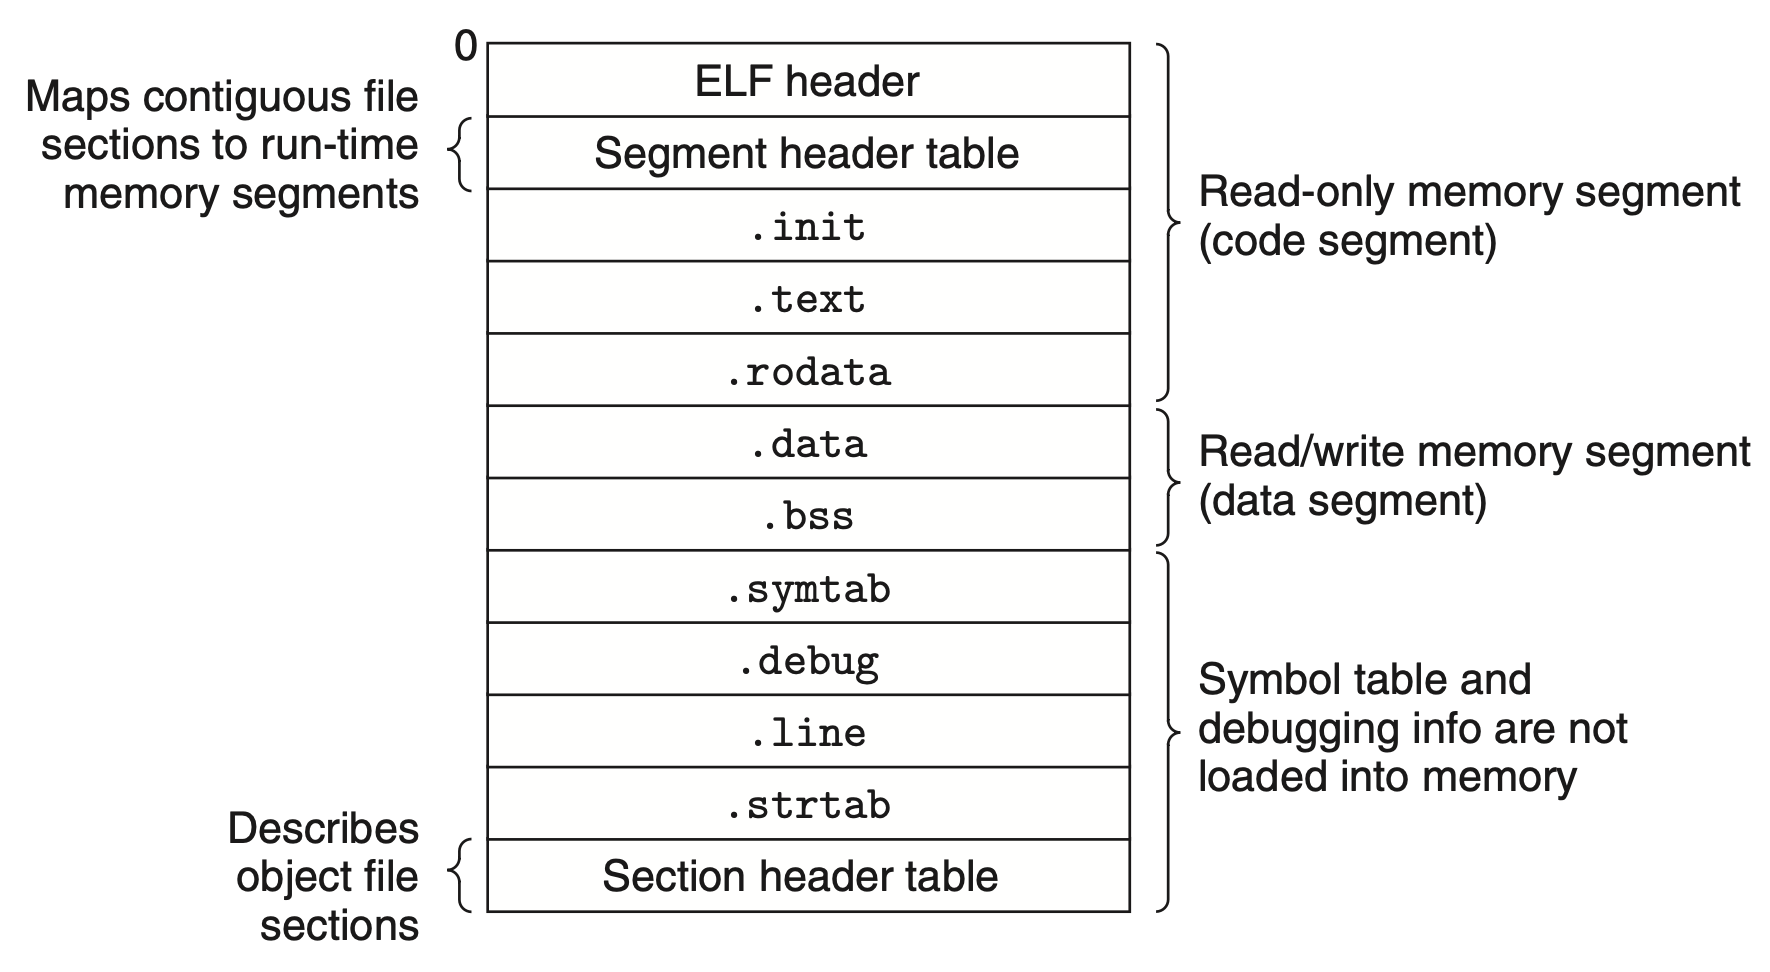
\includegraphics[width=0.75\textwidth]{day3/img/elf-layout-2.png}
			\caption{ELFs are organized into sections}
		\end{figure}
		%     \end{column}
		%     \begin{column}{0.2\textwidth}
		%         123
		%     \end{column}
		% \end{columns}
	}

	% \only<2>{
	%     \begin{tabular}{c|c|c}
	%         \hline
	%         \textbf{Section} & \textbf{W} & \textbf{X}\\
	%         \hline
	%         \verb|.text| & No & Yes \\
	%         \verb|.rodata| & No & No \\
	%         \verb|.data| & Yes & No \\
	%         \verb|.bss| & Yes & No \\
	%         \hline
	%     \end{tabular}
	% }
\end{frame}

\begin{frame}[fragile]{Process Address Space}
	\begin{columns}
		\begin{column}{0.3\textwidth}
			\begin{figure}[H]
				\centering
				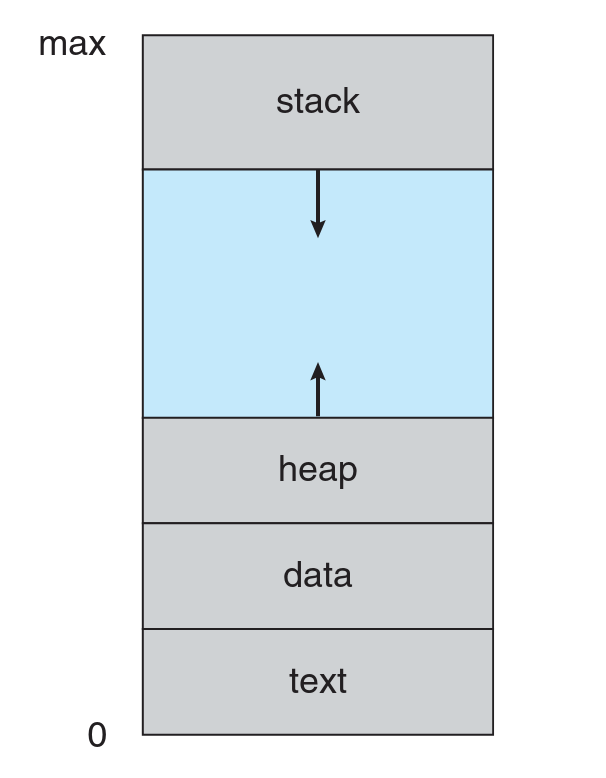
\includegraphics[width=\textwidth]{day3/img/process-layout.png}
			\end{figure}
		\end{column}
		\begin{column}{0.7\textwidth}
			A Process = A Program in Execution =
			\begin{itemize}
				\item<1-> \textbf{In Memory (Unique Address Space)}:
				      \begin{itemize}
					      \item \textbf{Code}: Text section, initially stored on disk
					      \item<2-> \textbf{Data Section}:
					            \begin{itemize}
						            \item \textbf{BSS}: Uninitialized data
						            \item \textbf{Data}: Initialized data
					            \end{itemize}
					      \item<3-> \textbf{Stack}: Function frames, local variables, etc.
					      \item<3-> \textbf{Heap}: Dynamic memory allocation
				      \end{itemize}
				\item<4-> \textbf{Context}:
				      \begin{itemize}
					      \item \textbf{Program Counter}: Points to the next instruction to execute (i.e., an address in the code)
					      \item Content of the processor's \textbf{registers}
				      \end{itemize}
			\end{itemize}
		\end{column}
	\end{columns}
\end{frame}

% \begin{frame}[fragile]{ELF Cheatsheet}
%     \begin{figure}[H]
%         \centering
%         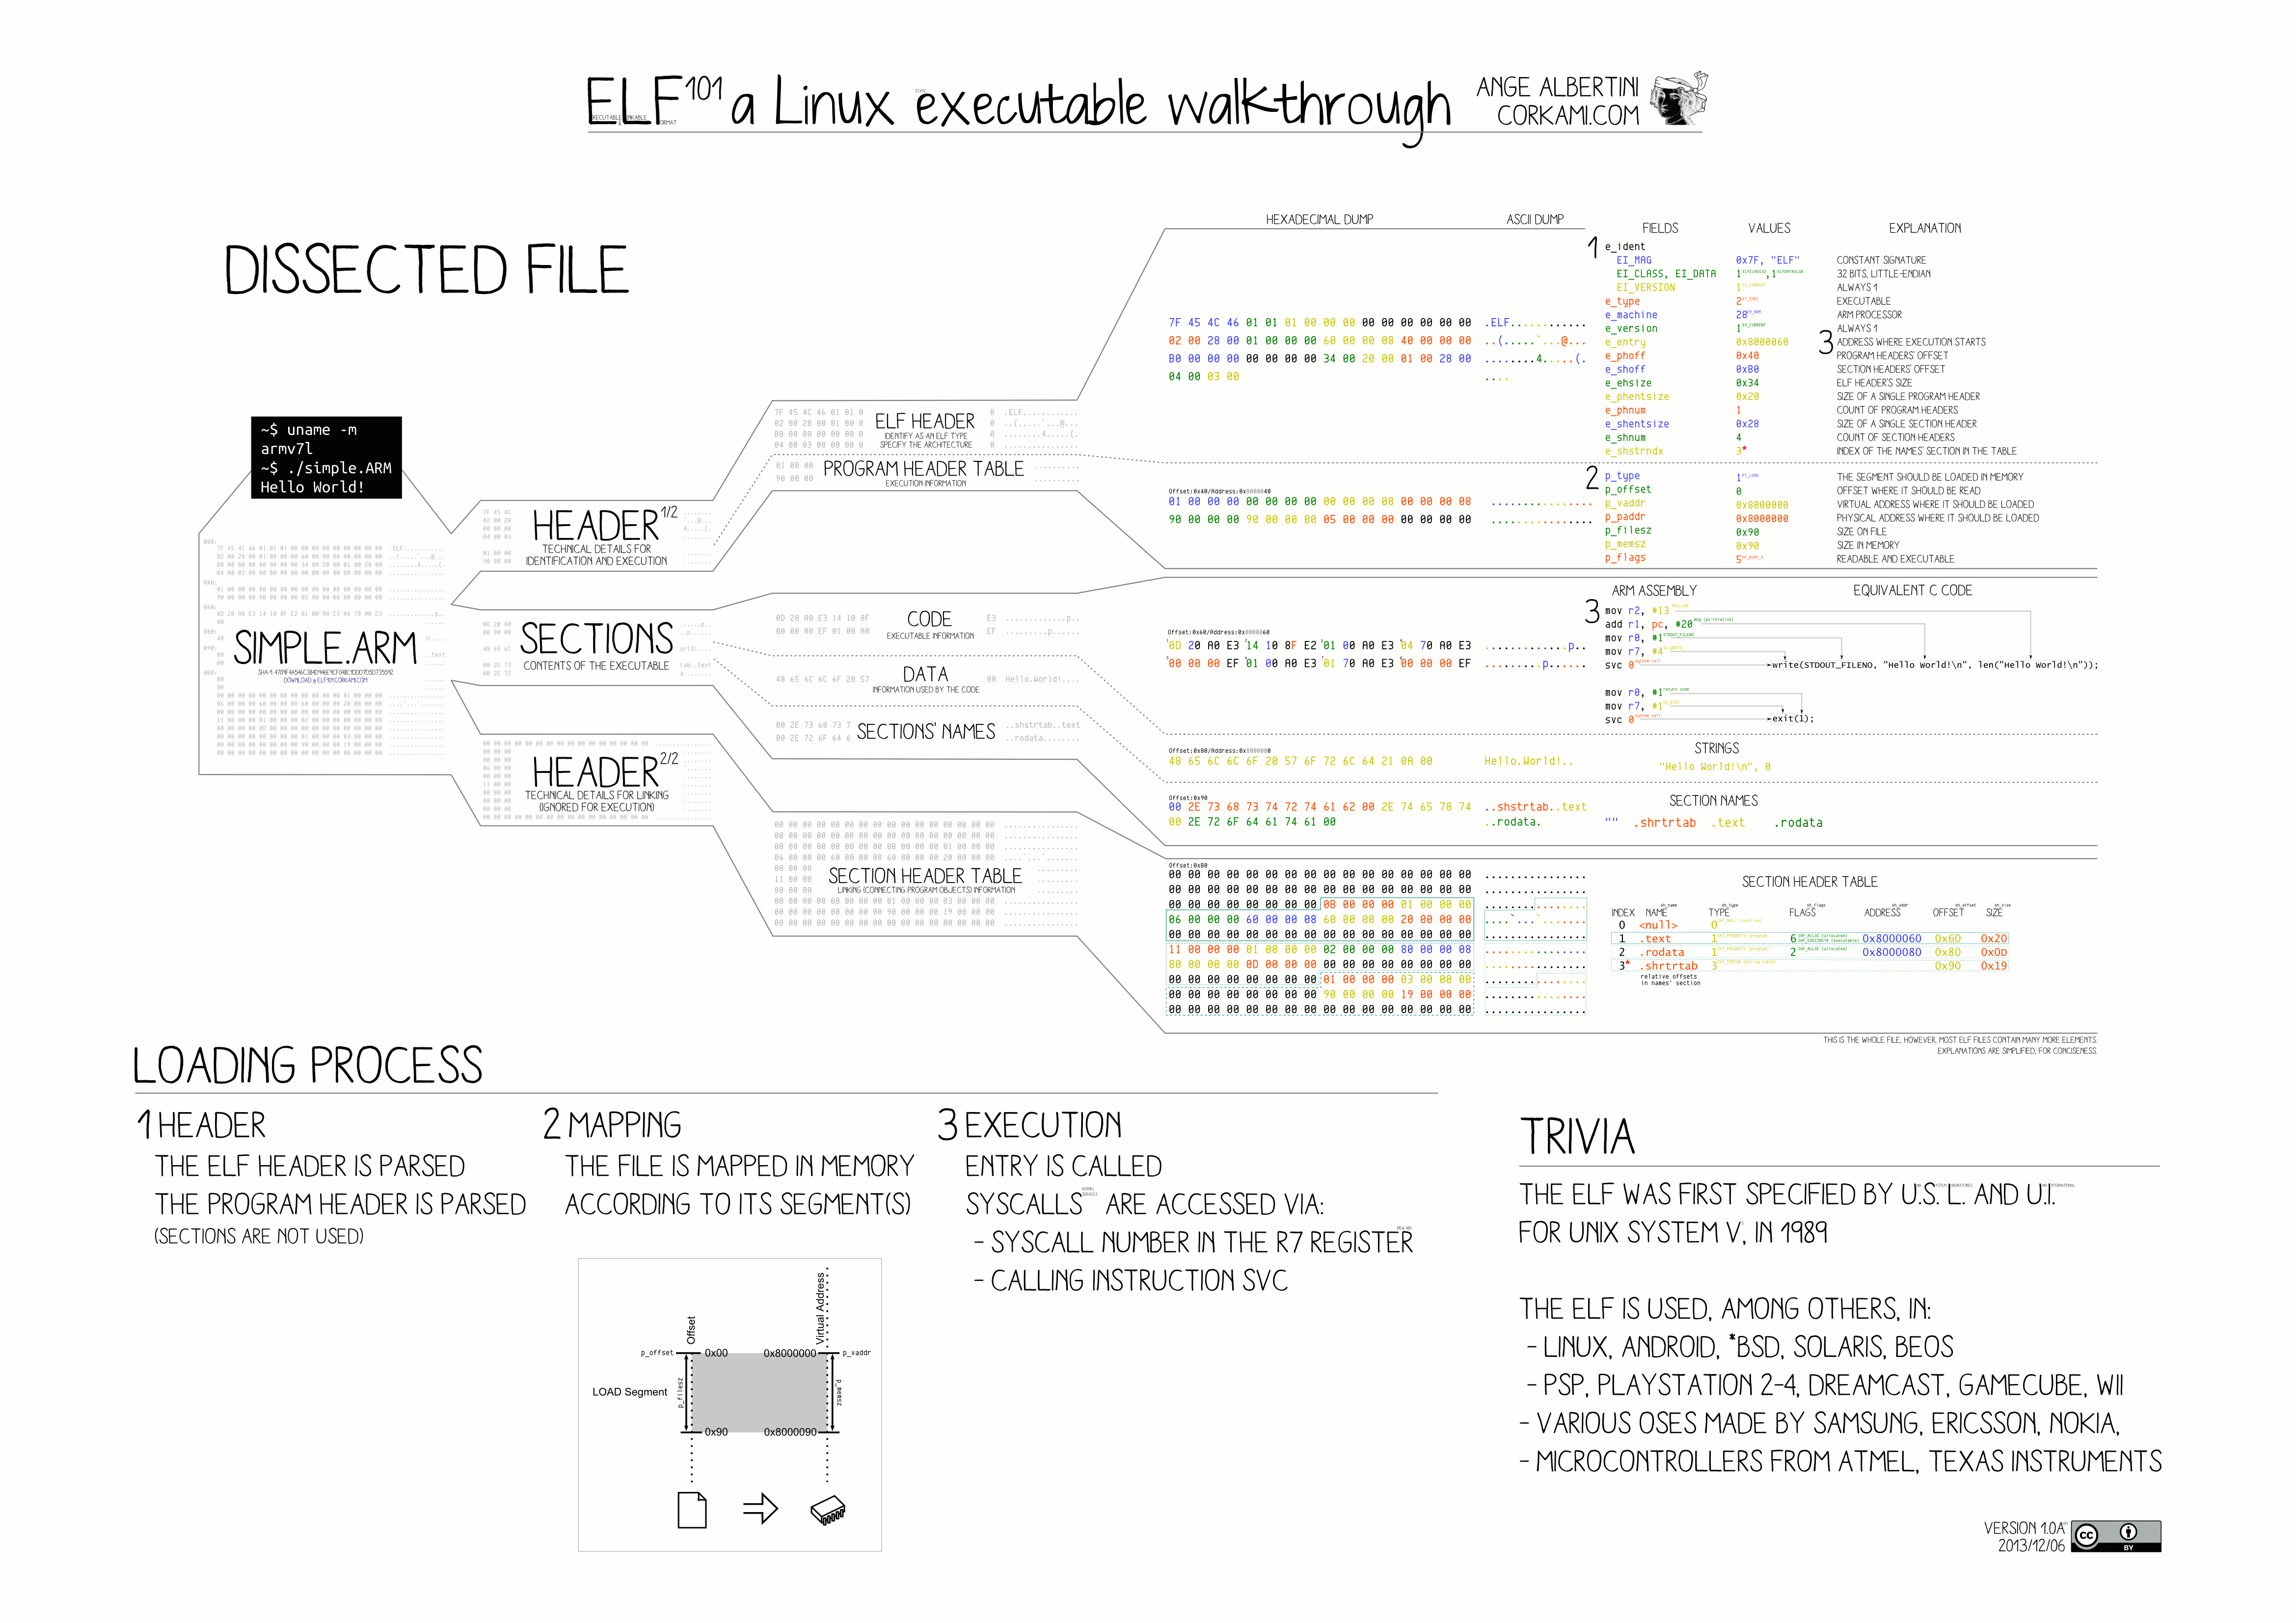
\includegraphics[width=\textwidth]{day3/img/elf-cheatsheet.png}
%     \end{figure}
% \end{frame}

\begin{frame}[fragile]{Stack Frame}
	\begin{figure}[H]
		\centering
		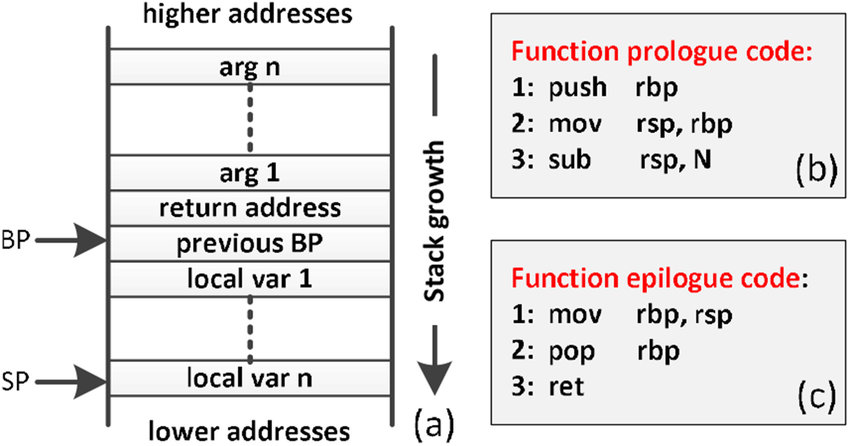
\includegraphics[width=0.8\textwidth]{day3/img/stack.jpg}
	\end{figure}
\end{frame}

\begin{frame}[fragile=singleslide,containsverbatim]{Quick Check: Memory Layout of C Program}
	Match the variables to the correct memory location:
	\begin{columns}
		\begin{column}{0.3\textwidth}
			\begin{figure}[H]
				\centering
				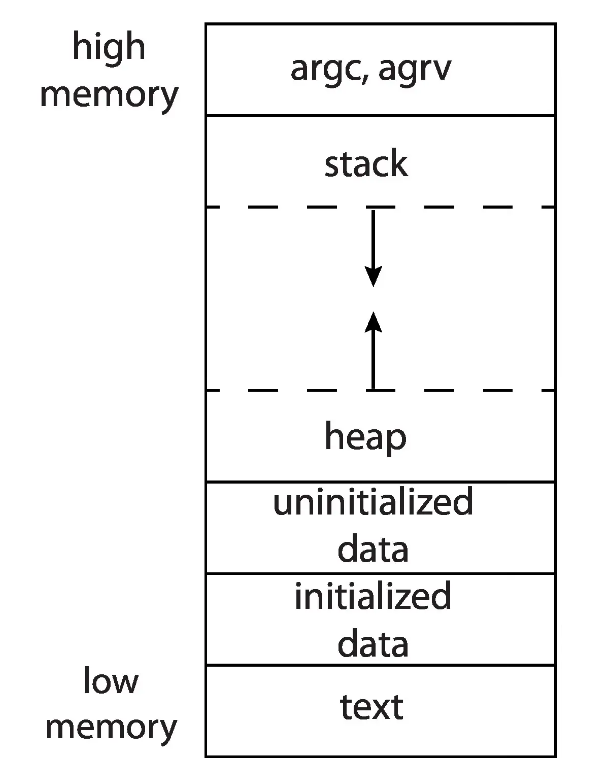
\includegraphics[width=\textwidth]{day3/img/mem-layout.png}
			\end{figure}
		\end{column}
		\begin{column}{0.7\textwidth}
			\begin{minted}[fontsize=\scriptsize,escapeinside=||]{c}
#include <stdio.h>
#include <stdlib.h>
int x;
int y = 15;
int main(int argc, char *argv[]) {
    int *values;
    int i;
    values = (int *)malloc(sizeof(int) * 5);
    for (i = 0; i < 5; i++)
        values[i] = i;
    return 0;
}
        \end{minted}
		\end{column}
	\end{columns}
\end{frame}

\begin{frame}[fragile=singleslide,containsverbatim]{Quick Check: Memory Layout of C Program (Answer)}
	\begin{figure}[H]
		\centering
		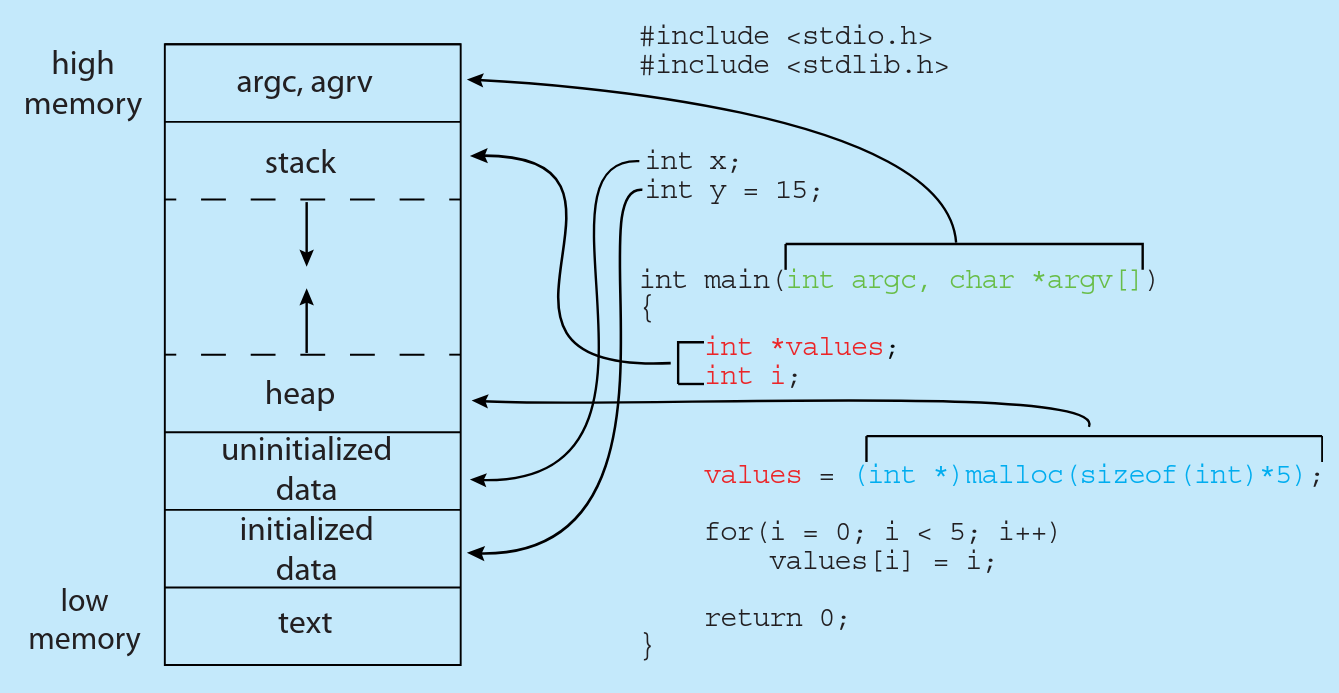
\includegraphics[width=0.9\textwidth]{day3/img/answer-layout.png}
	\end{figure}
\end{frame}

\subsection{Process Schedule}

\begin{frame}[fragile]{Process Schedule}
	\begin{itemize}
		\item \textbf{Non-preemptive}: The process must finish its execution before the OS can schedule another process.
		\item<2-> \textbf{Preemptive}: The OS can interrupt a process to schedule another one.
		      \begin{itemize}
			      \item<3-> Round Robin
			      \item<3-> Priority-based
		      \end{itemize}
	\end{itemize}
	\onslide<3->{
		\begin{figure}[H]
			\centering
			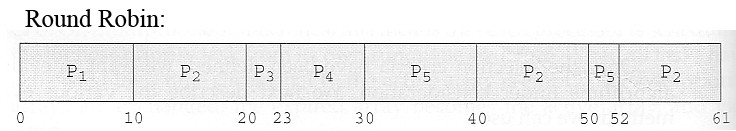
\includegraphics[width=0.6\textwidth]{day3/img/gantt.jpg}
		\end{figure}
		\begin{itemize}
			\item<4-> \emoji{star} \textbf{Also decide which process to run on which core.} (Control by \textbf{Core Affinity})
		\end{itemize}
	}
\end{frame}

\begin{frame}[fragile]{Process Switch}

	% Context Switch between two kernel processes:
	% \begin{figure}[ht!]
	%     \center
	%     \begin{tikzpicture}[x=0.8pt,y=0.8pt,yscale=-1,xscale=1]
	%     %uncomment if require: \path (0,300); %set diagram left start at 0, and has height of 300

	%     %Shape: Rectangle [id:dp0022237957984407863]
	%     \draw  [color={rgb, 255:red, 119; green, 187; blue, 221 }  ,draw opacity=1 ][fill={rgb, 255:red, 119; green, 187; blue, 221 }  ,fill opacity=0.05 ] (6,58.43) -- (438,58.43) -- (438,234.29) -- (6,234.29) -- cycle ;
	%     %Straight Lines [id:da4498626232311549]
	%     \draw [color={rgb, 255:red, 255; green, 136; blue, 153 }  ,draw opacity=1 ]   (38,123.43) -- (135,123.43) ;
	%     \draw [shift={(138,123.43)}, rotate = 180] [fill={rgb, 255:red, 255; green, 136; blue, 153 }  ,fill opacity=1 ][line width=0.08]  [draw opacity=0] (8.93,-4.29) -- (0,0) -- (8.93,4.29) -- cycle    ;
	%     %Straight Lines [id:da4226129673115242]
	%     \draw [color={rgb, 255:red, 255; green, 136; blue, 153 }  ,draw opacity=1 ]   (151.71,109.71) -- (140.12,121.31) ;
	%     \draw [shift={(138,123.43)}, rotate = 315] [fill={rgb, 255:red, 255; green, 136; blue, 153 }  ,fill opacity=1 ][line width=0.08]  [draw opacity=0] (8.93,-4.29) -- (0,0) -- (8.93,4.29) -- cycle    ;
	%     %Straight Lines [id:da24204008474623473]
	%     \draw [color={rgb, 255:red, 255; green, 136; blue, 153 }  ,draw opacity=1 ]   (138,123.43) -- (138,165) ;
	%     %Straight Lines [id:da12426250382299653]
	%     \draw [color={rgb, 255:red, 255; green, 136; blue, 153 }  ,draw opacity=1 ]   (138,165) -- (237.71,165) ;
	%     \draw [shift={(240.71,165)}, rotate = 180] [fill={rgb, 255:red, 255; green, 136; blue, 153 }  ,fill opacity=1 ][line width=0.08]  [draw opacity=0] (8.93,-4.29) -- (0,0) -- (8.93,4.29) -- cycle    ;
	%     %Straight Lines [id:da40164286447171516]
	%     \draw [color={rgb, 255:red, 119; green, 187; blue, 221 }  ,draw opacity=1 ]   (240.71,152.71) -- (240.71,177.29) ;
	%     %Straight Lines [id:da38281948784259523]
	%     \draw [color={rgb, 255:red, 119; green, 119; blue, 170 }  ,draw opacity=1 ]   (240.71,165.43) -- (316,165.43) ;
	%     %Straight Lines [id:da8211978963630775]
	%     \draw [color={rgb, 255:red, 119; green, 119; blue, 170 }  ,draw opacity=1 ]   (316,165.43) -- (316,144.43) ;
	%     \draw [shift={(316,141.43)}, rotate = 90] [fill={rgb, 255:red, 119; green, 119; blue, 170 }  ,fill opacity=1 ][line width=0.08]  [draw opacity=0] (8.93,-4.29) -- (0,0) -- (8.93,4.29) -- cycle    ;
	%     %Straight Lines [id:da9723145334004362]
	%     \draw [color={rgb, 255:red, 119; green, 119; blue, 170 }  ,draw opacity=1 ]   (316,141.43) -- (335,141.43) -- (418,141.43) ;
	%     \draw [shift={(421,141.43)}, rotate = 180] [fill={rgb, 255:red, 119; green, 119; blue, 170 }  ,fill opacity=1 ][line width=0.08]  [draw opacity=0] (8.93,-4.29) -- (0,0) -- (8.93,4.29) -- cycle    ;
	%     %Straight Lines [id:da6787843944387311]
	%     \draw [color={rgb, 255:red, 255; green, 136; blue, 153 }  ,draw opacity=1 ]   (209,180.86) -- (224.72,167.38) ;
	%     \draw [shift={(227,165.43)}, rotate = 139.4] [fill={rgb, 255:red, 255; green, 136; blue, 153 }  ,fill opacity=1 ][line width=0.08]  [draw opacity=0] (8.93,-4.29) -- (0,0) -- (8.93,4.29) -- cycle    ;
	%     %Straight Lines [id:da580092866214728]
	%     \draw [color={rgb, 255:red, 119; green, 119; blue, 170 }  ,draw opacity=1 ]   (298.71,124.14) -- (313.88,139.31) ;
	%     \draw [shift={(316,141.43)}, rotate = 225] [fill={rgb, 255:red, 119; green, 119; blue, 170 }  ,fill opacity=1 ][line width=0.08]  [draw opacity=0] (8.93,-4.29) -- (0,0) -- (8.93,4.29) -- cycle    ;

	%     % Text Node
	%     \draw (23,70.29) node [anchor=north west][inner sep=0.75pt]  [font=\normalsize,color={rgb, 255:red, 119; green, 187; blue, 221 }  ,opacity=1 ] [align=left] {Kernel Space};
	%     % Text Node
	%     \draw (47,107) node [anchor=north west][inner sep=0.75pt]  [font=\small] [align=left] {Kernel thread};
	%     % Text Node
	%     \draw (327,105) node [anchor=north west][inner sep=0.75pt]  [font=\small] [align=left] {Another\\Kernel thread};
	%     % Text Node
	%     \draw (153,98) node [anchor=north west][inner sep=0.75pt]  [font=\small,color={rgb, 255:red, 255; green, 136; blue, 153 }  ,opacity=1 ] [align=left] {Trap (timer)};
	%     % Text Node
	%     \draw (209,183.86) node [anchor=north] [inner sep=0.75pt]  [font=\small,color={rgb, 255:red, 255; green, 136; blue, 153 }  ,opacity=1 ] [align=left] {call switch\_to};
	%     % Text Node
	%     \draw (59,123) node [anchor=north west][inner sep=0.75pt]  [color={rgb, 255:red, 255; green, 136; blue, 153 }  ,opacity=1 ] [align=left] {dummy};
	%     % Text Node
	%     \draw (342,140.43) node [anchor=north west][inner sep=0.75pt]  [color={rgb, 255:red, 119; green, 119; blue, 170 }  ,opacity=1 ] [align=left] {dummy};
	%     % Text Node
	%     \draw (231,135) node [anchor=north west][inner sep=0.75pt]  [color={rgb, 255:red, 119; green, 187; blue, 221 }  ,opacity=1 ] [align=left] {ret};
	%     % Text Node
	%     \draw (128,167) node [anchor=north] [inner sep=0.75pt]  [font=\small,color={rgb, 255:red, 255; green, 136; blue, 153 }  ,opacity=1 ] [align=left] {P0 Trap Handler};
	%     % Text Node
	%     \draw (333,168) node [anchor=north] [inner sep=0.75pt]  [font=\small,color={rgb, 255:red, 255; green, 136; blue, 153 }  ,opacity=1 ] [align=left] {\textcolor[rgb]{0.47,0.47,0.67}{P1 Trap Handler}};
	%     % Text Node
	%     \draw (245,108) node [anchor=north west][inner sep=0.75pt]  [font=\small,color={rgb, 255:red, 119; green, 119; blue, 170 }  ,opacity=1 ] [align=left] {Trap exit};
	%     \end{tikzpicture}
	% \end{figure}
	\begin{figure}[H]
		\centering
		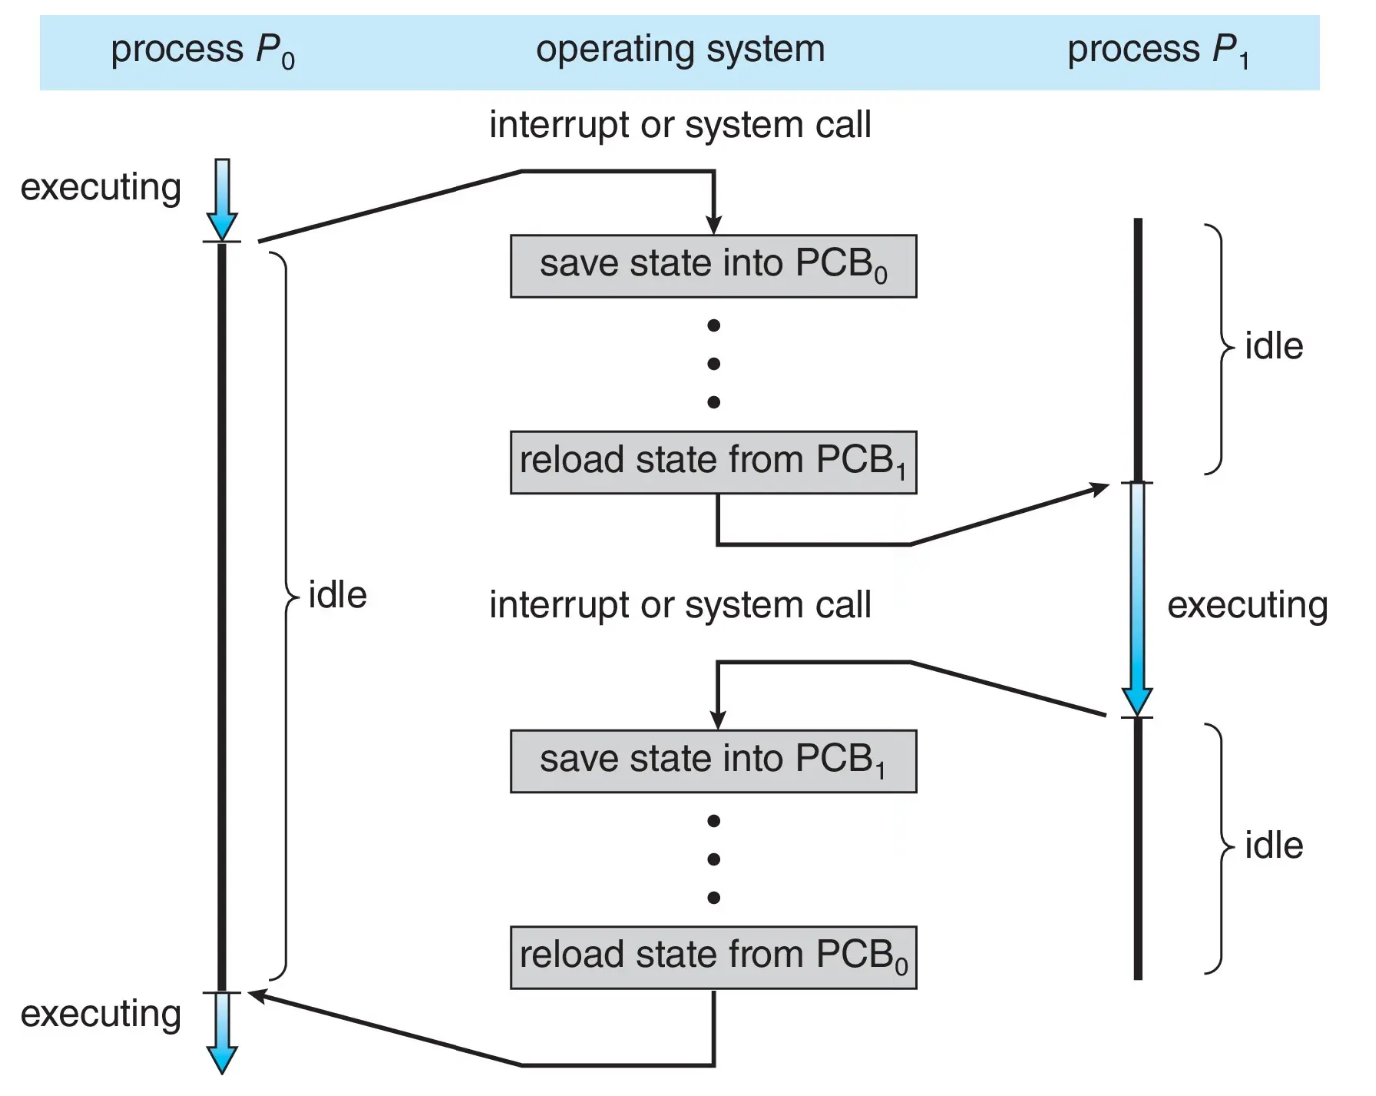
\includegraphics[width=0.6\textwidth]{day3/img/switch1.png}
	\end{figure}
\end{frame}


\subsection{Inter-Process Communication (IPC)}

\begin{frame}[fragile]{Inter-Process Communication}
	\only<1>{
		\textbf{Why?}
		\begin{itemize}
			\item Processes within a host may be \textbf{cooperating}
		\end{itemize}
		\begin{figure}[H]
			\centering
			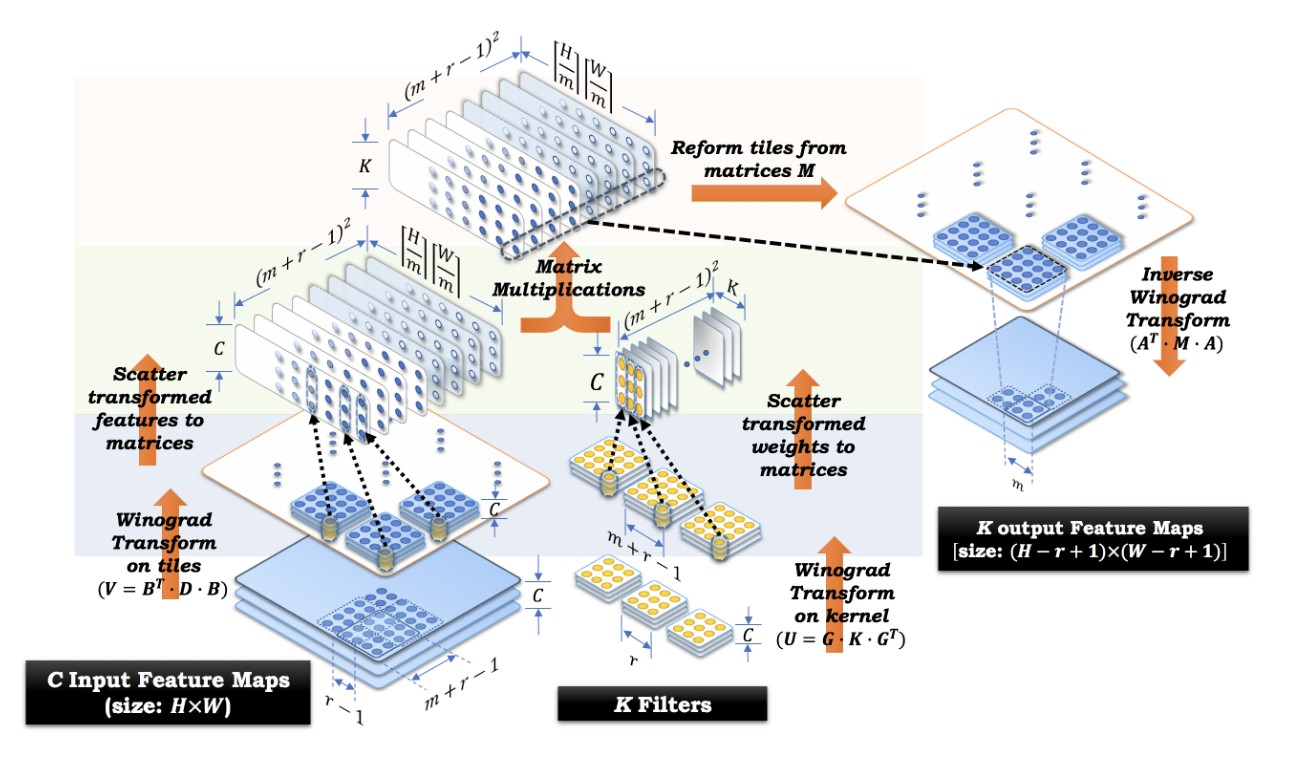
\includegraphics[width=0.65\textwidth]{day3/img/winograd.jpg}
		\end{figure}
	}

	\only<2>{
		\textbf{How?}
		\begin{itemize}
			\item \textbf{Message Passing}: We use \textbf{MPI} to send / receive messages.
			\item Shared Memory, Signal, Pipe, Socket...
		\end{itemize}
		\begin{figure}[H]
			\centering
			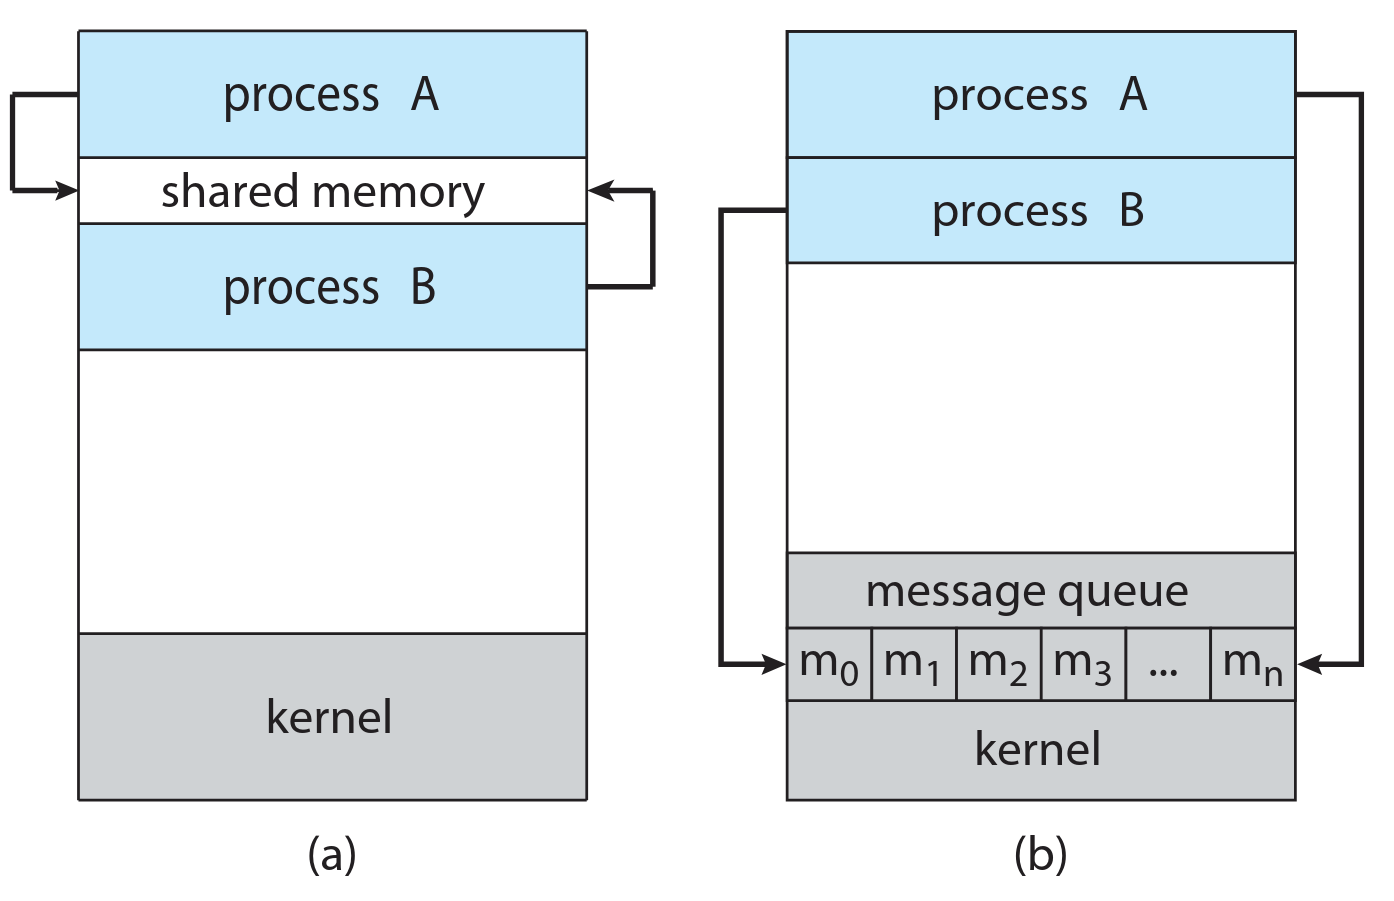
\includegraphics[width=0.5\textwidth]{day3/img/ipc.png}
		\end{figure}
	}
\end{frame}

\begin{frame}[fragile]{Inter-Process Communication}
	Disadvantages of IPC: \textbf{It's too heavy!} \emoji{woozy-face}
	\begin{itemize}
		\item Due to \textbf{isolation}, processes do not share address space.
		\item<2-> For message passing:
		      \begin{itemize}
			      \item Need to maintain a \textbf{message queue} for each process.
			      \item Data need to be \textbf{copied between address spaces}.
		      \end{itemize}
		\item<3-> For shared memory:
		      \begin{itemize}
			      \item Synchronization is needed
			      \item It's \textbf{complex for OS to manage}.
		      \end{itemize}
		\item<4-> Must flush cache when switching between processes. (Why?)
	\end{itemize}
	\onslide<5>{ \emoji{thinking} Is there a better way? }
\end{frame}
